\documentclass[11pt,a4paper]{article}

% ---------- Packages ----------
\usepackage[utf8]{inputenc}
\usepackage[T1]{fontenc}
\usepackage{lmodern}
\usepackage{geometry}
\usepackage{setspace}
\usepackage{booktabs}
\usepackage{array}
\usepackage{hyperref}
\usepackage{graphicx}
\usepackage{float}
\usepackage{csquotes}
\usepackage[title]{appendix}

% ---------- Page setup ----------
\geometry{
    margin=2.5cm
}

\setstretch{1.08}
\setlength{\parindent}{0pt}
\setlength{\parskip}{0pt}

\hypersetup{
    colorlinks=true,
    linkcolor=black,
    urlcolor=blue,
    citecolor=black,
    hypertexnames=false
}

% ---------- Title ----------
\title{
    \textbf{Philosopher Debate Arena}\\
    \large Design and Qualitative Evaluation of a Prompt-Conditioned Multi-Agent Debate System
}

\author{
    Sven Natterer \& Simon Rönner\\
    INF-3600 Generative Artificial Intelligence
}

\date{May 2026}

\begin{document}

\maketitle

\begin{abstract}
This report presents \emph{Philosopher Debate Arena}, an interactive multi-agent system designed to generate philosopher-inspired debates and balanced opinions using large language models. The system supports structured multi-round debates between two personas and a free topic opinion-generation mode, both of which can be orchestrated via single-agent prompts or a collaborative multi-agent team (two parallel strategists and a third agent acting as both the critic and final speaker). Additionally, the system incorporates automated judging and structured summaries. The project focuses on prompt-based persona conditioning, configurable argumentation strategies, and LLM-based evaluation rather than historical reconstruction. Qualitative evaluation indicates that the system produces coherent, stylistically distinct debate interactions, but highlights limitations regarding factual grounding, persona fidelity, judge reliability, and model-specific formatting stability.
\end{abstract}

\section{Introduction}

Large language models (LLMs) are capable of producing fluent argumentative text and can be conditioned through prompts to adopt particular roles, styles, and argumentative positions. These properties make them suitable for exploratory applications in which multiple model instances interact under different constraints. One possible application domain is philosophical debate, where contrasting positions, rhetorical style, and argumentative structure are central to the user experience.

This project investigates the use of prompt-conditioned LLM agents in an interactive debate and opinion-generation environment. The resulting Streamlit application, \emph{Philosopher Debate Arena}, allows users to configure and run debates or opinion queries using customizable philosopher personas, argumentation strategies, multi-agent team configurations, and automated evaluations.

The guiding research question is:

\begin{quote}
To what extent can prompt-conditioned LLM agents generate coherent, distinguishable, and interactive philosopher-inspired arguments in a configurable debate setting?
\end{quote}

The project has both technical and educational relevance. From a technical perspective, it examines prompt engineering, multi-agent orchestration, model routing, UI state management, and automated evaluation. From an educational perspective, it explores whether abstract philosophical positions can be made more accessible through interactive debate. The application should therefore be understood as an experimental system for generative interaction design rather than as an authoritative philosophical simulation.

\section{System Overview}

The system is implemented as a Streamlit application with a staged interaction flow, separating the user interface (state management, rendering) from the underlying debate engine (model execution, routing, judging, and text-to-speech audio generation). The functional responsibilities of the main system components are summarized in Table~\ref{tab:components}.

\begin{figure}[H]
\centering
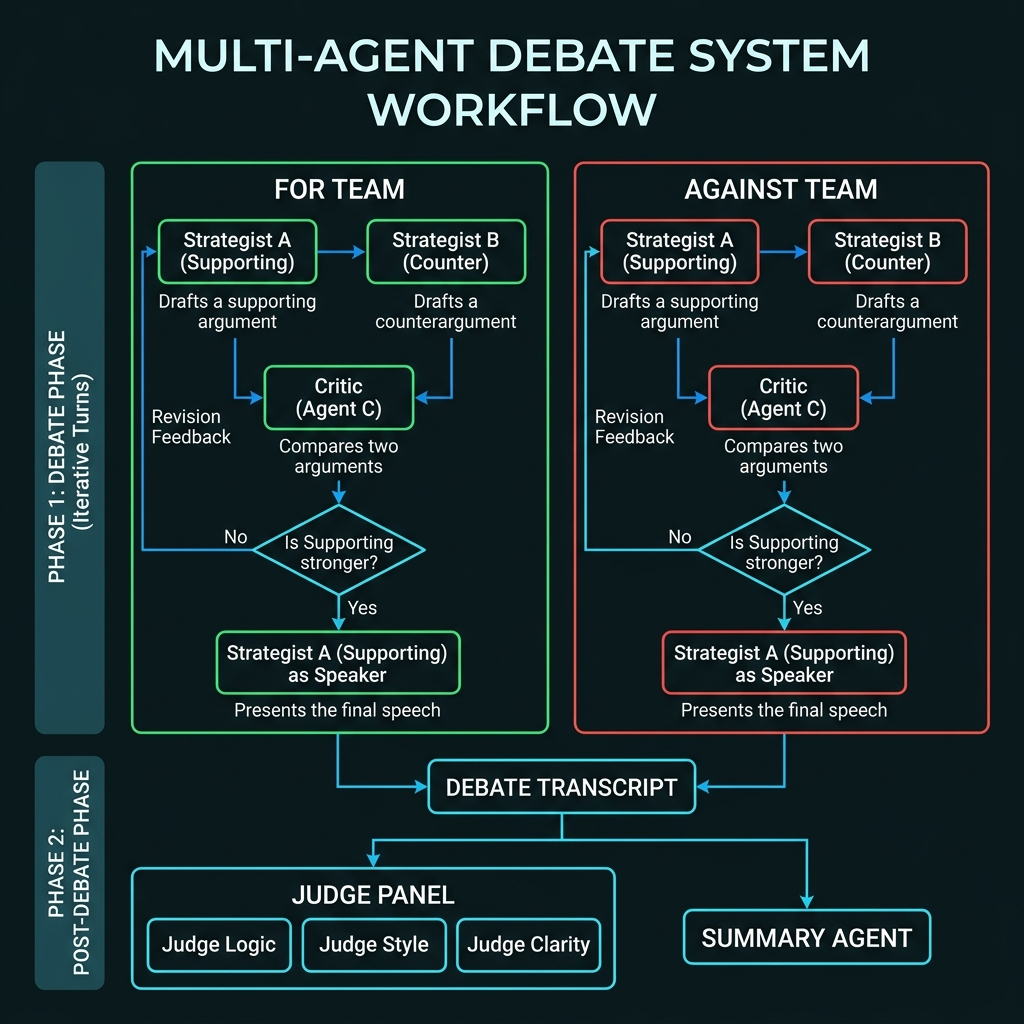
\includegraphics[width=0.75\textwidth]{agent_architecture.png}
\caption{System architecture and multi-agent interaction flow showing parallel strategist drafting, iterative critic critique-revision loops (where the critic also acts as the final speaker), and post-debate evaluation and summarization.}
\label{fig:agent_architecture}
\end{figure}


\subsection{Main Components}

\begin{table}[H]
\centering
\begin{tabular}{>{\raggedright\arraybackslash}p{4cm} >{\raggedright\arraybackslash}p{10cm}}
\toprule
\textbf{Component} & \textbf{Function} \\
\midrule
Streamlit frontend & Provides the staged user interface for settings, topic selection, character selection, live arena streaming, a dedicated summary stage, and diagnostics. \\
Philosopher library & Includes 20 philosopher-inspired personas with names, custom images, stances, speech voices, and style definitions. \\
Debate \& Team engine & Manages single-agent responses or orchestrates multi-agent teams (two strategists proposing arguments, and a third critic who evaluates them and acts as the speaker) in both Debate and Free Topic modes. \\
Strategy module & Converts user-selected strategies (logical, emotional, rhetorical, counterargument-oriented) into system instructions. \\
Judge panel & Evaluates debates using one to three concurrent judge agents with specific focus areas (logic, style, clarity, or general) and aggregates results. \\
Summary module & Automatically generates a concise sentence-by-sentence summary of the transcript at the final stage. \\
Developer diagnostics & Optionally logs and displays token usage and detailed multi-agent team traces. \\
Audio output & Generates neural text-to-speech audio via Microsoft Edge and plays it through local host audio channels with customized voices and stereo panning for each speaker. \\
\bottomrule
\end{tabular}
\caption{Functional overview of the system components.}
\label{tab:components}
\end{table}

\section{Methodology}

The project follows an implementation-oriented methodology. Instead of training a new model, it investigates how existing LLMs behave when embedded in a constrained interaction design. The implementation therefore focuses on prompt construction, role assignment, configurable model routing, and qualitative inspection of generated outputs.

\subsection{Technical Challenges and API Integration}

The integration of heterogeneous LLM backends highlighted the limits of achieving deterministic behavior and formatting. This manifested in two primary challenges:

First, \emph{formatting instability and model routing constraints} arose from heterogeneous model behaviors. Reasoning models (e.g., DeepSeek-R1, Phi-4) output internal thinking traces (within \texttt{<think>} blocks), and other models frequently ignored negative constraints by introducing redundant speaker headers or malformed XML tags. While a cleaning pipeline using regular expressions was implemented to remove these artifacts, the instability of very small models (e.g., the 1B parameter class) led to their removal. Enforcing JSON schemas (via the \texttt{instructor} library) on small models caused "schema collapse," and the text-cleaning filters proved insufficient to correct their erratic output formats. Consequently, very small models were excluded, restricting the local baseline to larger variants (e.g., Llama 3.2 3B) and relying on cloud models (e.g., GPT-4.1 mini) for components that strictly require structured output, such as the Judge. Additionally, safety-refusals in smaller aligned models when adopting provocative personas (like Nietzsche) required prompt adjustments or model routing.

Second, \emph{UI layout integration and system timeouts} required custom engineering. Injecting raw markdown paragraphs (separated by double newlines) into custom HTML blocks caused Streamlit to prematurely close containers and ruin CSS rendering; this was resolved by pre-converting markdown to HTML. Furthermore, loading larger models locally or waiting for deep reasoning traces often exceeded default 30-second API timeouts, requiring client timeouts to be extended to 180 seconds for overall stability.

\subsection{Supported Model Configurations}

The application supports a curated set of local and cloud-based models configured in the debate engine. The detailed specifications, roles, and backends of all active models are provided in Appendix~\ref{sec:appendix-models}.


\subsection{Evaluation Procedure}

The application was evaluated qualitatively through functional testing across its key configuration dimensions. The evaluation focused on assessing the stylistic recognizability and consistency of the 20 philosopher personas, the impact of the debate stance (for, against, or balanced), the differences between single-agent prompts and the multi-agent team mode (consisting of two parallel strategists and a critic-speaker), the influence of the argumentation strategies (logical, emotional, rhetorical, or counterargument-oriented), the effects of varying the number of debate rounds (one to five), and the stability and behavior of different model backends and judge panel configurations (one to three judge agents).

\section{Results}

Functional testing verified that the system successfully runs both debate and free topic flows, maintaining persona configurations and correctly displaying the outputs across the arena and summary stages. In multi-agent team mode, the critic-speaker and strategist-review loops successfully resolved safety refusals and aligned drafts to historical styles prior to display. The summary generator consistently reduced multi-round transcripts to a chronological sequence of single sentences. The judge panel successfully output structured scores and winners, with multi-judge configurations reducing individual model biases.

\section{Discussion}

The results demonstrate that prompt-conditioned LLM agents can be orchestrated into a structured, interactive debate environment. The main value of the system lies in its educational and exploratory UI, allowing users to configure settings (such as team mode, review loops, and argumentation strategies) to observe their impact on the generated arguments. 

The multi-agent team pattern (two parallel strategists and a critic-speaker) acts as a valuable structural guardrail. By introducing a critique-and-revision cycle, the team mode helps align responses to historical styles and mitigates safety-refusal issues common in highly-aligned cloud models. However, because the judge panel is also LLM-based, it may reward surface-level fluency and rhetorical confidence over genuine philosophical depth. Therefore, the judging and evaluation components are best understood as interactive features that enhance user engagement rather than as scientifically objective measuring instruments.

\section{Limitations}

Several limitations constrain the interpretation of the system.

First, the philosopher personas are generated through prompt conditioning rather than through retrieval from primary or secondary philosophical sources. This limits authenticity and makes the output sensitive to model pretraining biases. A philosopher-inspired agent may therefore reproduce popular associations rather than a nuanced reconstruction of the philosopher's work.

Second, the evaluation is qualitative and exploratory. The current report does not present a controlled user study, statistical comparison, or benchmark-based evaluation. As a result, claims about coherence, recognizability, and educational value should be understood as observations from system testing rather than as generalizable empirical findings.

Third, the system is sensitive to prompt wording and backend choice. Different models may produce substantially different levels of coherence, style consistency, and judgement quality. Reproducibility therefore requires careful documentation of selected models, prompts, settings, and debate topics.

Fourth, the host-side audio playback relies on the external Microsoft Edge TTS cloud API for high-quality neural voice generation. While it provides distinct voices and stereo-panning, it requires an active internet connection to download speech files and is dependent on the host machine's audio output devices.

\section{Future Work}

Future development should focus on grounding, evaluation, and richer interaction.

A retrieval-augmented generation component could improve philosophical authenticity by retrieving relevant passages from curated primary or secondary texts before each agent response. This would allow agents to refer to source material rather than relying solely on model-internal knowledge. Such a feature would require careful source selection, chunking, retrieval, citation handling, and prompt integration.

The evaluation methodology could be strengthened through human ratings. Participants could assess debate transcripts according to coherence, persona consistency, persuasiveness, educational value, and perceived authenticity. These ratings could then be compared with the judge agent's scores to investigate whether the automated evaluation aligns with human judgement.

The multi-agent team structure could also be extended. While each side can already utilize a team of two strategists and a critic-speaker, future versions could introduce specialized agents like a factual checker or a citation-lookup agent to verify historical accuracy before a response is finalized.

Finally, the audio system could be upgraded to fully local text-to-speech generation. Local models such as Kokoro or Piper could provide high-quality, consistent voices without requiring external cloud APIs, while expressive models or curated sound effects could support more theatrical presentation.

\section{Conclusion}

\emph{Philosopher Debate Arena} demonstrates how prompt-conditioned LLM agents can be combined with an interactive UI, configurable debate settings, automated judging, and optional diagnostics to create a complete multi-agent debate application. The system can generate coherent and stylistically varied philosopher-inspired exchanges, especially when persona, stance, strategy, and debate length are clearly constrained.

The application should not be interpreted as a historically accurate simulation of philosophers or as an objective evaluator of philosophical reasoning. Its primary contribution lies in demonstrating an interactive design pattern for generative AI systems: role-conditioned agents can be orchestrated into structured debates, inspected through a judge component, and exposed to users through adjustable settings. The project therefore provides a foundation for future work on grounded philosophical agents, richer multi-agent collaboration, and more rigorous evaluation of LLM-generated argumentative interaction.

\clearpage
\begin{appendices}
\section{Supported Model Configurations}
\label{sec:appendix-models}

The available model options configured in the system are summarized in Table~\ref{tab:models}:

\begin{table}[H]
\centering
\begin{tabular}{>{\raggedright\arraybackslash}p{3.5cm} >{\raggedright\arraybackslash}p{3.3cm} >{\raggedright\arraybackslash}p{7.2cm}}
\toprule
\textbf{Model Identifier (UI)} & \textbf{Provider\slash Backend} & \textbf{Role / Characteristics} \\
\midrule
Llama3.2:3b (Local) & Ollama (Local) & Zero-cost baseline for local testing and basic persona simulation. \\
GPT-4.1 mini (Platform) & Custom (Cloud) & Default model for structured tasks (e.g., automated judging). \\
GPT-5-chat (Platform) & Custom (Cloud) & Frontier model for high-fidelity argumentation and reasoning. \\
DeepSeek-V3.2 (Platform) & Custom (Cloud) & High-performance reasoning model for deep philosophical grounding. \\
Mistral Large 3 (Platform) & Custom (Cloud) & Commercial cloud model offering fluent, structured outputs. \\
Mistral Small (Platform) & Custom (Cloud) & Low-cost, fast model for lightweight cloud generation. \\
Llama 4 Maverick (Platform) & Custom (Cloud) & Open-weights instruction model optimized for fast responses. \\
Llama 3.3 70B (Platform) & Custom (Cloud) & Large-scale open-weights model for high-quality debates. \\
\bottomrule
\end{tabular}
\caption{Overview of active models available in the application.}
\label{tab:models}
\end{table}
\end{appendices}

\end{document}

